Als  Ausgangspunkt  der  Reglerdimensionierung dient  die  Schrittantwort  der
Strecke. Durch  Einzeichnen  der  Wendetangente\footnotemark[1]  ergeben  sich
Schnittpunkte  der  Wendetangente mit  der  Zeitachse  $[T_u,0]$ und  mit  dem
Zielwert $[T_g+T_g,K_s]$.   Es k\"onnen nun also  die Verz\"ogerungszeit $T_u$
und  die  Anstiegszeit   $T_g$  aus  Abbildung~\ref{fig:plant_step}  abgelesen
werden.

\footnotetext[1]{%
    Die Wendetangante ist die Tangente an den Wendepunkt in der Anstiegs-Phase
    der Schrittantwort.
}

Wir werden in diesem Bericht folgende Strecke als Beispiel nehmen:
\begin{figure}[h! width=\pagewidth]
    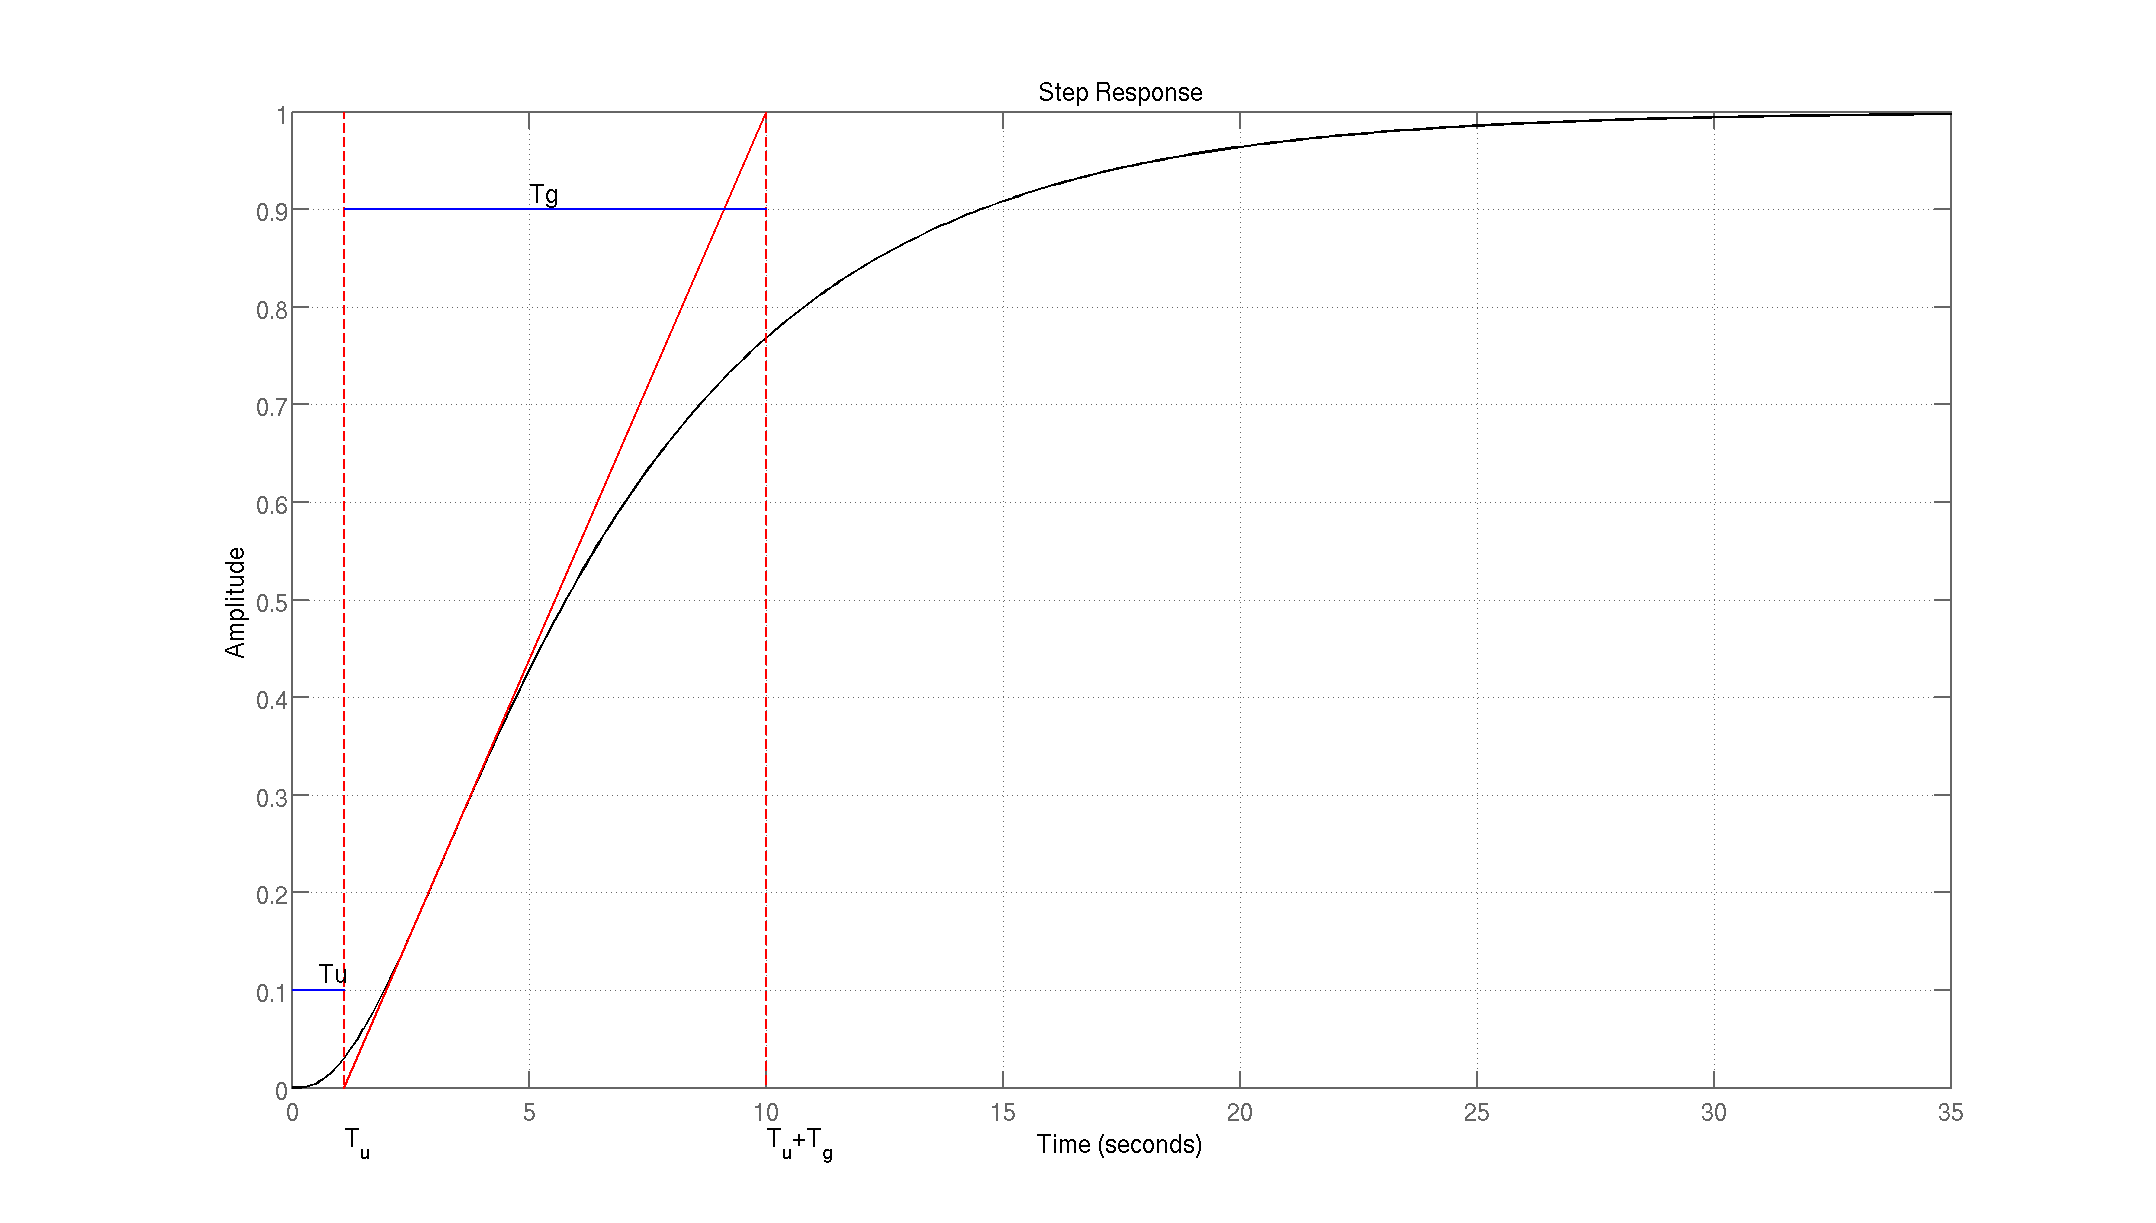
\includegraphics[width=\textwidth]{images/streckeSchrittantwort.png}
    \caption{%
    Schrittantwort der  Beispielstrecke (schwarz), Wendetangende  (rot), $T_u$
    und $T_g$ (blau)
    }
    \label{fig:plant_step}
\end{figure}

Ausmessen der Schrittantwort ergibt:
\begin{itemize}
    \item
        $K_s = 2$\footnotemark[2]
    \item
        $T_u = \SI{1.1}{\second}$
    \item
        $T_g = \SI{8.9}{\second}$
\end{itemize}

\footnotetext[2]{%
    Abbildung~\ref{fig:plant_step}  ist  auf  1  normiert,  die  Verst\"arkung
    unserer  Beispielstrecke   betr\"agt  $2$.    An  den  Werten   f\"ur  die
    Verz\"ogerungs-  und Anstiegszeit  oder  am  Ausmessen der  Schrittantwort
    \"andert sich dadurch nichts
}

Der  geschlossene   Regelkreis  soll  schlussendlich  maximal   etwa  $16.3\%$
\"uberschwingen.

Da  die  Reglerdimensionierung  mit  der  Phasengangmethode  vom  Frequenzgang
einer  Strecke  ausgeht und  nicht  von  deren  Schrittantwort, wird  aus  den
obigen Werten  nun der Frequenzgang  der Strecke bestimmt.  Dies  erledigt die
Methode  \code{p\_sani()}\footnotemark[3],  welche  uns die  Werte  f\"ur  die
\"Ubertragungsfunktion  der  Strecke liefert.   In  unserem  Fall ergibt  dies
folgendes Polynom:

\footnotetext[3]{%
    Die  Methode  \code{p\_sani()} wurde  zu  Beginn  des Projektes  in  einer
    Matlab-Implementation  vom  Auftraggeber   zur  Verf\"ugung  gestellt  und
    anschliessend f\"ur unser Tool in Java \"ubersetzt.

    Sie kann aus der Verz\"ogerungszeit, der Anstiegszeit und der Verst\"arkung
    der Strecke ein Polynom f\"ur deren \"Ubertragungsfunktion vom Grad 1 bis 8
    ausrechnen.

    Als Eingabeparameter werden  die Werte $T_u$, $T_g$  und $K_s$ ben\"otigt,
    als R\"uckgabewert erh\"alt  man ein Array mit den Zeiten  $T_i$ f\"ur die
    Nenner der Faktoren des Polynoms (siehe Gleichung~\ref{eq:transfer:plant}).

    Genauere  Informationen  zur   Funktionsweise  von  \code{p\_sani()}  sind
    Anhang~\ref{app:sani} zu entnehmen.
}

\begin{gather} \label{eq:transfer:plant}
    \begin{split}
        H_s (s) & = K_s
                  \cdot \frac{1}{1 + s \cdot T_1}
                  \cdot \frac{1}{1 + s \cdot T_2}
                  \cdot \frac{1}{1 + s \cdot T_2}                     \\
                & = 2
                  \cdot \frac{1}{1 + s \cdot \SI{0.4134}{\second}}
                  \cdot \frac{1}{1 + s \cdot \SI{1.4894}{\second}}
                  \cdot \frac{1}{1 + s \cdot \SI{5.3655}{\second}}
    \end{split}
\end{gather}

Mit   einem  geeigneten   Tool  kann   man  sich   den  dazugeh\"origen   Plot
(Abbildung~\ref{fig:plant_freq}) erstellen lassen.

\begin{figure}[h! width=\pagewidth]
    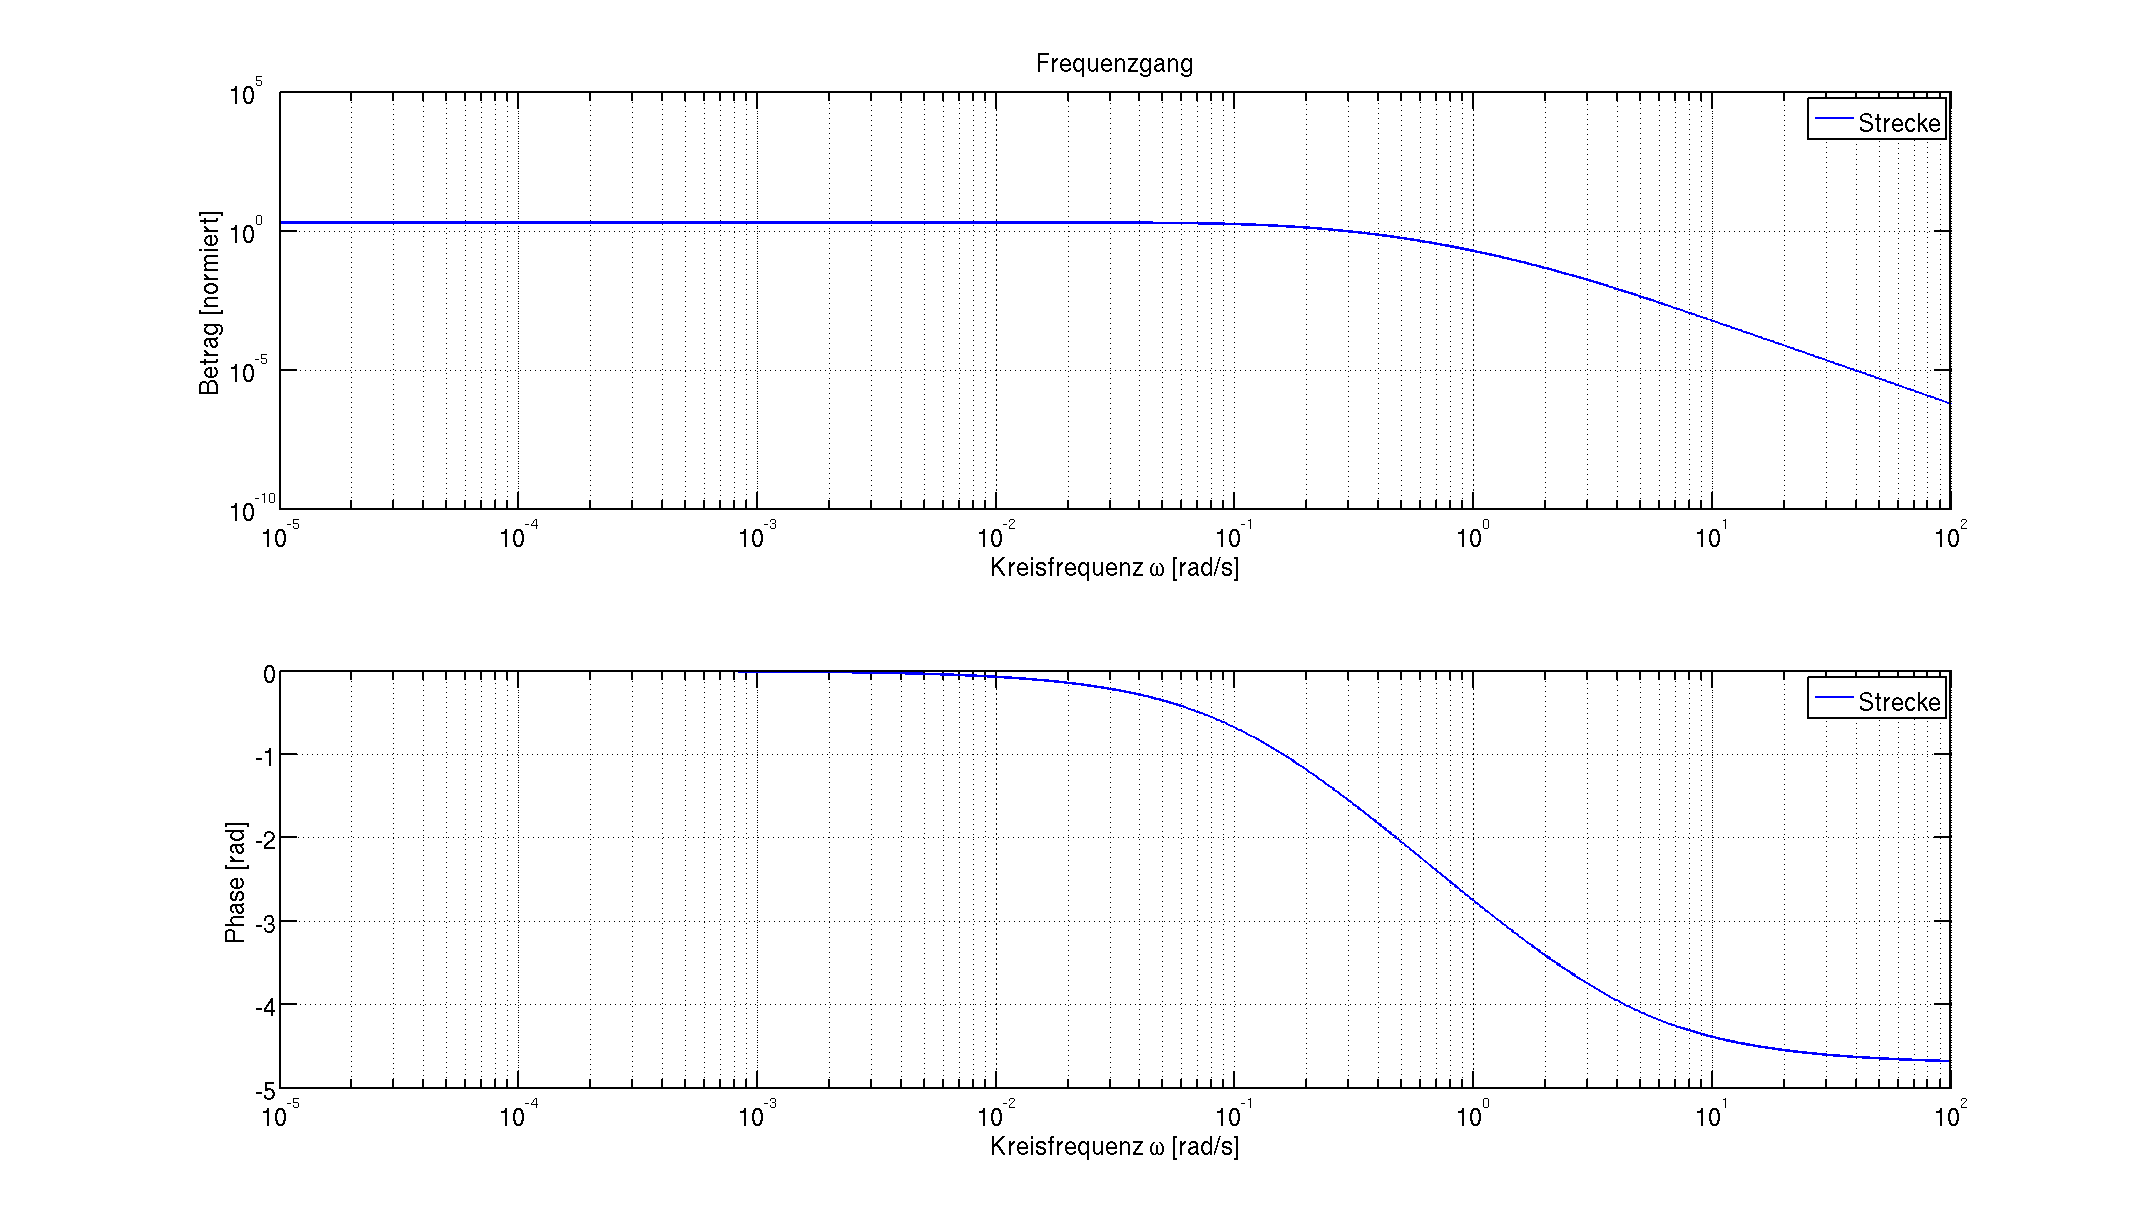
\includegraphics[width=\textwidth]{images/streckeFrequenzgang.png}
    \caption{%
        Frequenzgang der Strecke, mit Amplitudengang und Phasengang
    }
    \label{fig:plant_freq}
\end{figure}

Somit ist der Frequenzgang der Strecke bekannt und man hat alle erforderlichen
Informationen, um den Regler mit der Phasengangmethode zu dimensionieren.
